% A plain-English tour of the optimization model in optimization/explore.ipynb.
% Exact formulas and tables are in the appendices.
% Every equation, constant and bound below was read from the notebook's code cells
% (and, for the planing balance, from the installed OpenPlaning 0.4.9 source).
% Build:  tectonic explore-model.tex     (or: pdflatex explore-model.tex, twice)
\documentclass[11pt,a4paper]{article}

\usepackage[margin=2.2cm]{geometry}
\usepackage{amsmath,amssymb}
\usepackage{booktabs,longtable,array,tabularx}
\usepackage{enumitem}
\usepackage{float}
\usepackage{needspace}
\usepackage{xcolor}
\usepackage{tikz}
\usetikzlibrary{arrows.meta,positioning,calc}
\usepackage[hidelinks]{hyperref}
\usepackage{fancyhdr}

\setlength{\parindent}{0pt}
\setlength{\parskip}{0.7em}
\linespread{1.08}
\renewcommand{\arraystretch}{1.18}
\setlist{itemsep=0.15em,topsep=0.25em}
\pagestyle{fancy}
\fancyhf{}
\fancyhead[L]{\small Boat model of \texttt{explore.ipynb}}
\fancyhead[R]{\small\thepage}
\renewcommand{\headrulewidth}{0.3pt}

% --- shorthand ---------------------------------------------------------------
\renewcommand{\_}{\textunderscore\allowbreak}
\newcommand{\code}[1]{\texttt{#1}}
\newcommand{\unit}[1]{\,\mathrm{#1}}
\newcommand{\Trace}{T_{\mathrm{race}}}
\newcommand{\Pshaft}{P_{\mathrm{shaft}}}
\newcommand{\Pbus}{P_{\mathrm{bus}}}
\newcommand{\Eused}{E_{\mathrm{used}}}
\newcommand{\Epack}{E_{\mathrm{pack}}}
\newcommand{\Voc}{V_{\mathrm{oc}}}
\newcommand{\Vload}{V_{\mathrm{load}}}
\newcommand{\Vend}{V_{\mathrm{end}}}
\newcommand{\Rpack}{R_{\mathrm{pack}}}
\newcommand{\lcg}{\mathrm{LCG}}
\newcommand{\vcg}{\mathrm{VCG}}
\newcommand{\note}[1]{\par\smallskip\noindent\textbf{Note.} #1}


\title{How the boat model works\\[0.4em]
\large A plain-English tour of \texttt{explore.ipynb}}
\author{}
\date{\today}

\begin{document}
\maketitle
\thispagestyle{fancy}

\section*{The question}

We want a boat that covers two miles as fast as possible. This document explains the model in \code{explore.ipynb} that tries to find one.

The trouble is that everything depends on everything else. A faster boat needs more power. More power needs a bigger motor and a bigger battery.
Those make the boat heavier. A heavier boat needs more power to go the same speed. So you can't choose the motor first and the battery second.
You have to choose them together, along with the shape of the hull, and then see whether the whole thing works.

That is what the model does. You give it a complete design. It works out how much the boat weighs, where the weight sits, how hard the water pushes back,
how much power that takes and how much battery that uses. Then it checks the design against twenty rules. If the design passes, the model tells you how long the race would take.

One warning. Nothing here has been checked against a real boat. The battery cells, the motor weights and the propeller efficiency are all placeholders.
So read the answers as ``what the model believes,'' not ``what the boat will do.'' The model is more useful for something else: it shows which limits bite first,
and which choices matter.

\section*{What we get to choose}

There are ten choices, of four kinds. The shape of the hull: length, beam (the width), deadrise (the angle of the V on the bottom) and depth.
Where the payload and the battery sit along the hull. The motor: its power and its efficiency. And the battery: how many cells go in series, and how many of
those strings go in parallel. Series sets the voltage. Parallel sets the capacity, and how much current the pack can supply.

Eight of the ten vary continuously between bounds. The two battery counts are whole numbers.

\begin{table}[H]
\centering\small
\caption{Searched decision variables. Bounds are the notebook's \code{BOUNDS}; the baseline is the default \code{Design}.}
\label{tab:decisions}
\begin{tabularx}{\textwidth}{@{}l l l l l c X@{}}
\toprule
Symbol & Code name & Unit & Type & Bounds & Baseline & Group \\
\midrule
$L$        & \code{length\_ft}    & ft   & continuous & $[3,\ 10]$       & 8.5  & hull \\
$b$        & \code{beam\_in}      & in   & continuous & $[10,\ 40]$      & 16   & hull (chine beam) \\
$\beta$    & \code{deadrise\_deg} & deg  & continuous & $[6,\ 16]$       & 10   & hull \\
$D$        & \code{depth\_in}     & in   & continuous & $[8,\ 20]$       & 12   & hull \\
$\xi_p$    & \code{payload\_x}    & --   & continuous & $[0.25,\ 0.50]$  & 0.30 & placement (fraction of $L$ forward of transom) \\
$\xi_b$    & \code{battery\_x}    & --   & continuous & $[0.25,\ 0.45]$  & 0.35 & placement (fraction of $L$ forward of transom) \\
$P_m$      & \code{motor\_kw}     & kW   & continuous & $[2,\ 10]$       & 4.0  & motor rated shaft power \\
$\eta_m$   & \code{motor\_eff}    & --   & continuous & $[0.85,\ 0.95]$  & 0.90 & motor peak efficiency \\
$S$        & \code{series}        & --   & integer    & $\{12,13,14\}$   & 14   & battery series cells \\
$n_p$      & \code{parallel}      & --   & integer    & $\{1,\dots,12\}$ & 6    & battery parallel strings \\
\bottomrule
\end{tabularx}
\end{table}

Speed is missing from the list, and you might expect it to be there. It isn't, because for any given design there is a fastest speed at which every rule
still holds, and nobody would run slower. So we don't ask the search to pick a speed. For each design, the model finds that speed itself and uses it.
This turns the question into a simpler one: which design has the highest legal top speed?

The notebook has three more fields that the search leaves alone: propeller pitch, propeller diameter and thrust angle. Pitch and diameter change only some numbers the model
prints, because propeller efficiency is a fixed constant. Thrust angle does affect the balance, but it is held at zero.

\section*{How the model works out the rest}

Think of it as a chain. Each link uses what came before. Figure~\ref{fig:flow} shows the order.

\begin{figure}[t]
\centering
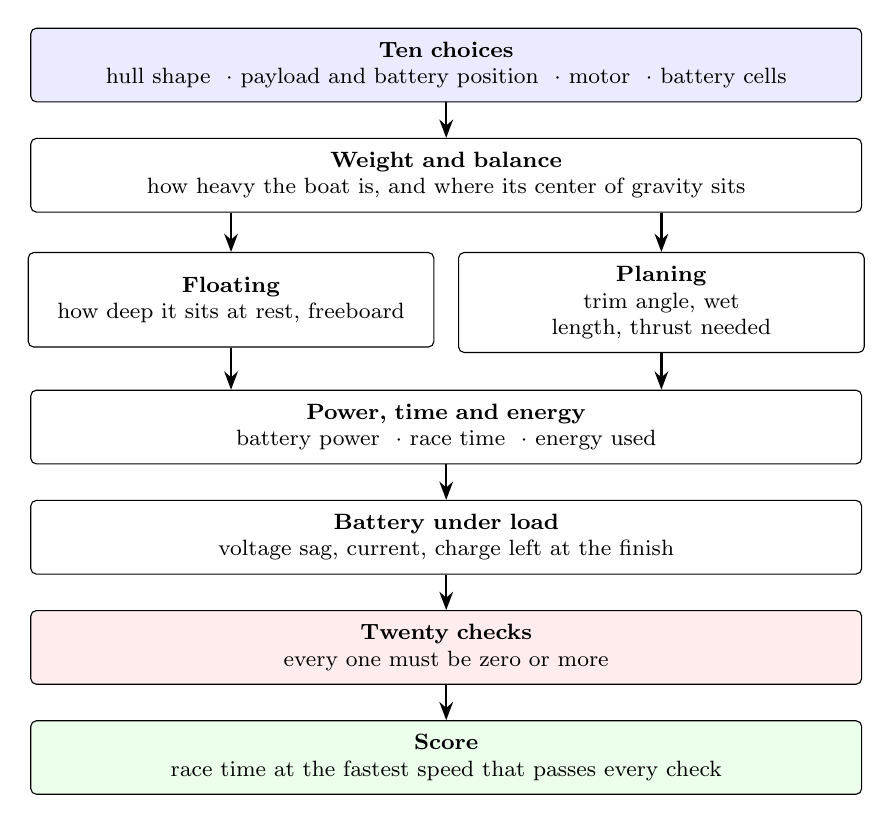
\begin{tikzpicture}[
  >=Stealth,
  box/.style={draw, rounded corners=2pt, align=center, font=\footnotesize, inner sep=5pt, text width=10.2cm},
  half/.style={draw, rounded corners=2pt, align=center, font=\footnotesize, inner sep=5pt, text width=4.8cm, minimum height=1.2cm},
  arr/.style={->, thick}]
  \node[box, fill=blue!8] (dec) {\textbf{Ten choices}\\ hull shape \ $\cdot$\ payload and battery position \ $\cdot$\ motor \ $\cdot$\ battery cells};
  \node[box, below=0.45cm of dec] (mass) {\textbf{Weight and balance}\\ how heavy the boat is, and where its center of gravity sits};
  \node[half, anchor=north east] (hydro) at ([xshift=-0.15cm, yshift=-0.5cm]mass.south) {\textbf{Floating}\\ how deep it sits at rest, freeboard};
  \node[half, anchor=north west] (plan) at ([xshift=0.15cm, yshift=-0.5cm]mass.south) {\textbf{Planing}\\ trim angle, wet length, thrust needed};
  \node[box, anchor=north] (power) at ($(hydro.south)!0.5!(plan.south)-(0,0.5cm)$) {\textbf{Power, time and energy}\\ battery power \ $\cdot$\ race time \ $\cdot$\ energy used};
  \node[box, below=0.45cm of power] (batt) {\textbf{Battery under load}\\ voltage sag, current, charge left at the finish};
  \node[box, below=0.45cm of batt, fill=red!7] (cons) {\textbf{Twenty checks}\\ every one must be zero or more};
  \node[box, below=0.45cm of cons, fill=green!8] (obj) {\textbf{Score}\\ race time at the fastest speed that passes every check};
  \draw[arr] (dec) -- (mass);
  \draw[arr] (hydro.north |- mass.south) -- (hydro.north);
  \draw[arr] (plan.north |- mass.south) -- (plan.north);
  \draw[arr] (hydro.south) -- (hydro.south |- power.north);
  \draw[arr] (plan.south) -- (plan.south |- power.north);
  \draw[arr] (power) -- (batt);
  \draw[arr] (batt) -- (cons);
  \draw[arr] (cons) -- (obj);
\end{tikzpicture}
\caption{What happens to one design at one speed.}
\label{fig:flow}
\end{figure}

\paragraph{Weight and balance.} Start with weight. The hull's weight is its surface area times the weight of the fiberglass per square foot, plus a fixed allowance for structure.
The battery's weight is the number of cells times the weight of one cell, plus 15\% for the case and wiring. The motor's weight comes from a made-up formula in which more power and
more efficiency both make it heavier. That stops the search from simply picking the biggest, best motor. Add the 30~lb payload, the propeller and 8.8~lb of fixed equipment,
and you have the total.

Each part sits somewhere along the hull and at some height above the keel. Averaging by weight gives the center of gravity. Where it sits front to back matters a lot, as you'll see.

\paragraph{Floating.} Next, how deep the boat sits when it's stopped. The model finds the draft at which the displaced water weighs as much as the boat, using the hull's cross-section.
Subtract the draft from the hull's depth and you get freeboard: how much hull is above the water. A planing boat rides higher once it's moving, so this is the cautious number.

\paragraph{Planing.} Now the hard part. At speed, a boat like this lifts up and skims across the water. Where it settles is a balance. The water has to push up with a force equal to the boat's weight,
and it has to do that without tipping the bow up or down. The angle the boat settles at is called trim. How much of the hull stays wet depends on trim, and the drag depends on how much is wet.

We don't work this out ourselves. A library called OpenPlaning does it, using a method published by Savitsky. We give it the weight, the center of gravity, the beam, the deadrise and the speed.
It gives back the trim, how much of the hull is wet, and the thrust the propeller must supply to keep going. For the default boat at about 22~mph the thrust is 110 newtons, and 97 of those are skin friction.
At this size most of the drag is just water rubbing along the bottom.

\paragraph{Power, time and energy.} Thrust times speed is the useful work the boat does each second. The propeller wastes some of it; we assume it is 65\% efficient. The motor wastes some more; the default motor is 90\% efficient.
Add 30 watts for electronics. What comes out is the power the battery must supply. The default boat needs about 1.9 kilowatts.

Race time is distance divided by speed. We use speed over the ground, which is the speed through the water minus a 1~mph current, and add 20 seconds of allowance. Energy used is power times that time.
The 20 seconds is charged at full cruise power, which is simple rather than realistic.

\paragraph{The battery.} The battery has two quirks. First, the competition caps pack voltage at 55.5 volts when fully charged. Fourteen cells in series would reach 58.8 volts when full, so the model charges the pack only as far as the cap allows.
For the default boat that is 75.5\%. This is computed, not chosen.

Second, a battery's voltage sags when you draw current from it, because of its internal resistance. More strings in parallel share the load and sag less. The model solves for the voltage under load, then the current,
then how much charge and what cell voltage remain at the finish.

\section*{What the boat has to obey}

The model checks twenty things. Each is a number that has to be zero or more. We call it a margin: how much room is left before the rule is broken. A design is feasible if all twenty margins are nonnegative.
They come in four kinds. The exact formulas are in Appendix~\ref{sec:constraints}; here is what they mean.

\paragraph{Competition rules (three).} Freeboard at rest must be at least 3 inches, plus half the 4-inch wave height, so 5 inches in all. The full-charge pack voltage must be at most 55.5 volts.
And the boat must make headway against the current.

\paragraph{Being a boat (one).} The hull must be deeper than the height of its chine, the edge where the bottom meets the sides. Otherwise there is no hull above the chine to speak of.

\paragraph{Hardware and balance (nine).} A fully charged pack must not exceed the motor's voltage rating. The race may use at most 70\% of the energy in the pack at the start. Shaft power must stay under 80\% of the motor's rating,
and current under 80\% of both the battery's and the motor's ratings. That 20\% cushion is a design margin. The pack must be able to deliver the power at all; past a certain draw the voltage equation has no solution.
Each cell must stay above 3.0 volts at the finish. And the center of gravity must sit between 30 and 45 percent of the hull's length from the back.

\paragraph{Staying inside the method (seven).} Savitsky's formulas were fitted to experiments over a limited range, and outside it the library is guessing. So the model treats the edge of that range as a wall.
The solver must find a balance at all. Trim must be between 2 and 15 degrees. The wetted length can be at most four beam-widths. A speed number built from speed and beam must lie between 0.6 and 13.
And the wetted keel can't be longer than the hull.

Six of the twenty don't depend on speed at all: freeboard, hull depth, both voltage checks and both center-of-gravity checks. They decide whether a design has any legal speed.
The other fourteen get harder as speed rises, and together they set the top speed.

\section*{What we minimise}
\label{sec:objective}

Race time, and nothing else. There is no cost term, and no goal for weight beyond the limits above.

For one design, the model finds the top speed like this. Try 8~mph, then 12, 16 and so on up to 60. Remember the highest speed at which all twenty checks pass. Then narrow in on the edge by repeated halving
until it is pinned down to a tenth of a mile per hour. The race time at that speed is the design's score. (Inside the search the scan is coarser, to be quicker.)

If no speed passes, the design gets a score of 1000 plus a measure of how badly it breaks the rules at 20~mph. That nudges the search toward designs that work.

To search over designs we use differential evolution: keep a population of candidate designs, mix and mutate the good ones, keep the improvements. The notebook runs it with three different random seeds.
It is a good way to explore, but it doesn't prove that no better design exists. If three seeds agree, that is reassuring, not conclusive.

Part II of the notebook also tries other ways of searching the same space (random search, dual annealing and a local search), and two other objectives.
Both of those fix the speed at a target of 25~mph and ask a different question of the same twenty checks. One asks for the lightest boat that can run that speed. The other asks for the boat
that uses the least energy over the course at that speed. An infeasible design scores 1000 plus 100 times how badly it breaks the rules. Race time stays the main objective, and the rest of this document is about it.

\section*{An example}

Take the default design: 8.5~ft long, 16-inch beam, 10-degree deadrise, a 4~kW motor, 14 cells in series and 6 strings. It weighs 82~lb. Its top speed is 22.56~mph, and its race time is 354 seconds,
under six minutes. The project's benchmark is seven.

\begin{table}[H]
\centering\small
\caption{Calculated values for the baseline design at $v^\star=22.56$ mph.}
\begin{tabular}{@{}l r l @{\qquad} l r l@{}}
\toprule
Quantity & Value & Unit & Quantity & Value & Unit \\
\midrule
hull mass $m_{\mathrm{hull}}$ & 20.43 & lb  & thrust $T$ & 110.1 & N \\
battery mass $m_{\mathrm{bat}}$ & 14.88 & lb & running trim $\tau$ & 2.002 & deg \\
motor mass $m_{\mathrm{mot}}$ & 7.40 & lb   & wetted length / beam $\lambda$ & 3.216 & -- \\
total mass $m$ & 82.01 & lb                  & beam speed coeff.\ $C_v$ & 5.052 & -- \\
$\lcg/L$ & 0.3373 & --                       & shaft power $\Pshaft$ & 1708 & W \\
pack energy $\Epack$ & 1512 & Wh            & bus power $\Pbus$ & 1928 & W \\
start charge $s_0$ & 75.5 & \%              & race time $\Trace$ & 353.9 & s \\
$\Voc$ & 55.5 & V                           & energy used $\Eused$ & 189.5 & Wh \\
static draft & 2.34 & in                     & loaded voltage $\Vload$ & 54.26 & V \\
freeboard & 9.66 & in                        & bus current $I$ & 35.5 & A \\
rated current $I_{\mathrm{rated}}$ & 88.2 & A & end charge $s_{\mathrm{end}}$ & 63.0 & \% \\
$I_{\lim}$ & 90 & A                          & end voltage $\Vend$ & 52.77 & V \\
\bottomrule
\end{tabular}
\end{table}

Now ask what stops it going faster. It isn't the motor, which is using about half of what it's allowed. It isn't the battery, which is using about half its allowed current and about a quarter of its allowed energy.
What stops it is trim. At 22.56~mph the boat's trim is 2.002 degrees, and the method's floor is 2. Go a little faster and the boat flattens below 2 degrees, where the formulas are no longer trusted.

So the model says the top speed is where its own method stops being valid. That is an uncomfortable answer, because it says nothing about the hardware. Appendix~\ref{sec:constraints} lists all twenty margins for this design.

\section*{What to doubt}
\label{sec:caveats}

\begin{itemize}
  \item \textbf{The speed limit comes from the method, not the boat.} Trim binds first, so nothing after it in the chain (drag, power, energy) gets a chance to bind. That is why the made-up numbers there look unimportant.
        They would matter if the trim floor were relaxed.
  \item \textbf{Nothing stops the boat from being narrow.} There is no rule about stability, packaging or ride. The notebook reports that its searches take the narrowest beam and a high deadrise. When a variable ends up on its bound,
        the model is telling you it is missing a rule.
  \item \textbf{Most inputs are placeholders.} The cell data, the motor weight formula, propeller efficiency, the hull's fullness (prismatic coefficient), the wave height, the current, the heights of components and the laminate weights.
        Appendix~\ref{sec:fixed} marks each one.
  \item \textbf{One check is zero by construction.} The charge level is chosen so the pack voltage lands exactly on 55.5 volts, so for 14 cells the voltage margin is zero up to rounding. It passes only because the arithmetic rounds the right way.
        A check written as ``at least zero'' on a number that is zero by design is fragile.
  \item \textbf{Propeller pitch and diameter do nothing.} With a constant propeller efficiency they change only numbers the model prints. Wave height matters only through freeboard.
  \item \textbf{The speed scan trusts the highest passing speed.} It doesn't check that the speeds below it also pass. A design that passes at 12 and 20~mph but not at 16 would be scored at about 20.
  \item \textbf{Two small quirks.} Turning off the validity checks (\code{ENFORCE\_VALIDITY = False}) lets a design whose planing solve failed count as feasible; the default is on. And the score of 1000 for infeasible designs
        is only safely worse than feasible ones above about 8.35~mph, since slower boats take more than 1000 seconds.
\end{itemize}

\section*{What to replace next}

Real cell data first: resistance, continuous current and the voltage curve. Then a real motor weight formula and voltage rating, a propeller model, and the hull's fullness. Then the wave height and current for the actual venue,
and real component heights. The notebook leaves out transom beam, bow deadrise and keel curve because OpenPlaning can't use them.

\appendix
\section{The formulas, in order}
\label{sec:calculated}
% =============================================================================

These are the exact formulas behind the chain described in the main text, in the order the notebook computes them. Nothing here is
chosen. Every value follows from the ten decisions, the constants in Appendix~\ref{sec:fixed} and the values before it.

\subsection{Hull geometry and mass}
The hull is prismatic: a V-bottom section of chine beam $b$ and deadrise $\beta$ with vertical sides up to the depth $D$,
the same from transom to bow. With $b_{\mathrm{ft}}=b/12$ and $t=\tan\beta$, the chine sits at height
\begin{equation}
  h_c = \tfrac12\, b_{\mathrm{ft}}\, t \quad[\mathrm{ft}] \qquad (\code{chine\_height\_ft}),
  \label{eq:chine}
\end{equation}
and the side height above the chine is $s_h = \max(D/12 - h_c,\ 0)$. The shell area is the sum of bottom, two sides, deck and transom:
\begin{equation}
  A_{\mathrm{shell}} = \underbrace{\frac{b_{\mathrm{ft}}L}{\cos\beta}}_{\text{bottom}}
  + \underbrace{2\,s_h L}_{\text{sides}} + \underbrace{b_{\mathrm{ft}}L}_{\text{deck}}
  + \underbrace{b_{\mathrm{ft}}s_h + \tfrac12 b_{\mathrm{ft}}h_c}_{\text{transom}} \quad[\mathrm{ft}^2],
  \qquad
  m_{\mathrm{hull}} = \rho_{\mathrm{lam}}\,A_{\mathrm{shell}} + m_{\mathrm{str}} \quad[\mathrm{lb}].
  \label{eq:hull}
\end{equation}

\subsection{Battery pack}
With $n = S\,n_p$ cells,
\begin{equation}
  \Epack = n\,q_c\,V_{\mathrm{nom}}\ [\mathrm{Wh}], \quad
  m_{\mathrm{bat}} = n\,m_c(1+\kappa_o)\ [\mathrm{lb}], \quad
  \Rpack = \frac{S}{n_p}\,r_c\ [\Omega], \quad
  I_{\lim} = n_p\,I_{c,\max}\ [\mathrm A].
  \label{eq:pack}
\end{equation}
Series cells add resistance and parallel strings share it, so more parallel strings reduce voltage sag.

\paragraph{Start-of-race charge (derived, not chosen).}
The pack starts at the highest state of charge at which its open-circuit voltage stays at or below the voltage rule, capped at 100\%:
\begin{equation}
  s_0 =
  \begin{cases}
    1 & S\,V_{\mathrm{full}} \le V_{\lim},\\[2pt]
    \mathrm{OCV}^{-1}\!\bigl(V_{\lim}/S\bigr) & \text{otherwise},
  \end{cases}
  \qquad
  \Voc = S\cdot\mathrm{OCV}(s_0).
  \label{eq:soc0}
\end{equation}
For the baseline, $S=14$ gives $14\times4.2=58.8>55.5\,\mathrm V$, so the pack is charged only to $s_0=75.5\%$ and $\Voc=55.5\,\mathrm V$.
For $S=12,13$ the pack starts full.

\subsection{Motor and propeller}
\begin{equation}
  m_{\mathrm{mot}} = (1 + 1.6\,P_m)\bigl(1 + 6(\eta_m - 0.90)\bigr)\ [\mathrm{lb}], \qquad
  I_{\mathrm{rated}} = \frac{1000\,P_m}{\eta_m\,S\,V_{\mathrm{nom}}}\ [\mathrm A].
  \label{eq:motor}
\end{equation}
The mass fit is a placeholder: it rises with rated power and with efficiency so the search cannot simply take the biggest,
most efficient motor. The rated bus current $I_{\mathrm{rated}}$ uses the \emph{nominal} pack voltage.
Reported propeller numbers (diagnostics only, no constraint):
\begin{equation}
  \mathrm{rpm} = \frac{1056\,v}{p\,\sigma_s}, \qquad
  v_{\mathrm{tip}} = \pi\,\frac{d_p}{12}\,\frac{\mathrm{rpm}}{60}\ [\mathrm{ft/s}], \qquad
  K_v = \frac{\mathrm{rpm}}{\Vload}.
  \label{eq:prop}
\end{equation}

\subsection{Mass and balance}
The boat is six point masses. With $x$ the fraction of $L$ forward of the transom and $z$ the height above the keel:

\begin{center}\small
\begin{tabular}{@{}l l l l@{}}
\toprule
Component $i$ & Mass $m_i$ (lb) & Position $x_i$ & Height $z_i$ (in)\\
\midrule
hull    & $m_{\mathrm{hull}}$ \eqref{eq:hull} & $0.45$   & $\zeta_h D$ \\
payload & $m_{\mathrm{pay}}=30$               & $\xi_p$  & $z_{\mathrm{pay}}=8$ \\
battery & $m_{\mathrm{bat}}$ \eqref{eq:pack}  & $\xi_b$  & $z_{\mathrm{bat}}=4$ \\
motor   & $m_{\mathrm{mot}}$ \eqref{eq:motor} & $0.10$   & $z_{\mathrm{mot}}=4$ \\
propeller & $m_{\mathrm{prop}}=0.5$           & $0.00$   & $z_{\mathrm{mot}}=4$ \\
fixed equipment & $m_{\mathrm{fix}}=8.8$      & $0.40$   & $z_{\mathrm{fix}}=8$ \\
\bottomrule
\end{tabular}
\end{center}
\begin{equation}
  m = \sum_i m_i, \qquad
  \frac{\lcg}{L} = \frac{\sum_i m_i x_i}{m}\ \ (\lcg\ \text{in ft}), \qquad
  \vcg = \frac{\sum_i m_i z_i}{m}\ [\mathrm{in}], \qquad
  r_g = \kappa_g L.
  \label{eq:balance}
\end{equation}
The 30~lb payload, propeller and fixed equipment are constants, so total mass moves with the hull, battery and motor.

\subsection{Hydrostatics}
Freeboard is measured at rest, which is conservative because the boat rides higher when planing.
The section area at draft $T$ (ft) is
\begin{equation}
  A_{\mathrm{sec}}(T) =
  \begin{cases}
    T^2/t & T \le h_c,\\
    \tfrac12 b_{\mathrm{ft}}h_c + b_{\mathrm{ft}}(T - h_c) & T > h_c.
  \end{cases}
  \label{eq:section}
\end{equation}
The static draft inverts this for the displaced volume $m/\rho_w$:
\begin{equation}
  A^\ast = \frac{m/\rho_w}{C_p\,L},\qquad
  T_{\mathrm{stat}} =
  \begin{cases}
    \sqrt{A^\ast t} & A^\ast \le \tfrac12 b_{\mathrm{ft}}h_c,\\[2pt]
    h_c + \dfrac{A^\ast - \tfrac12 b_{\mathrm{ft}}h_c}{b_{\mathrm{ft}}} & \text{otherwise},
  \end{cases}
  \qquad
  \text{freeboard} = D - 12\,T_{\mathrm{stat}}\ [\mathrm{in}].
  \label{eq:draft}
\end{equation}

\subsection{Planing equilibrium (OpenPlaning)}
\label{sec:planing}
For a given speed the boat is assumed to run at the trim and wetted length where lift balances weight and pitching
moments balance. The notebook builds an OpenPlaning \code{PlaningBoat} from SI versions of the quantities above:
\begin{align*}
  U &= 0.44704\,v, &
  W &= 4.44822\,m, &
  \text{beam} &= 0.0254\,b, &
  \text{lcg} &= 0.3048\,\lcg_{\mathrm{ft}},\\
  \text{vcg} &= 0.0254\,\vcg, &
  r_g &= 0.3048\,\kappa_g L, &
  \rho &= 16.01846\,\rho_w, &
  v_T &= 0.0254\cdot 4,
\end{align*}
with deadrise $\beta$, thrust angle $\varepsilon=0$, thrust longitudinal offset $0$ and kinematic viscosity $\nu$.
(The wave height $H_w$ is passed as \code{H\_sig}, but the notebook only calls the steady-trim and force routines, which do
not use it; wave height therefore affects the model only through the freeboard allowance.)

Let $F_{n}=U/\sqrt{g\,b}$ be the beam speed coefficient (the notebook's \code{cv}) and $\lambda=(L_K+L_C)/(2b)$ the mean wetted
length over beam, where $L_K$ and $L_C$ are the keel and chine wetted lengths that follow from the trim $\tau$ and the
waterline height. OpenPlaning's hydrodynamic force is Savitsky's planing-lift relation:
\begin{align}
  C_{L0} &= \tau^{1.1}\Bigl(0.012\,\lambda^{1/2} + 0.0055\,\frac{\lambda^{5/2}}{F_n^2}\Bigr), &
  C_{L\beta} &= C_{L0} - 0.0065\,\beta\,C_{L0}^{\,0.6},\nonumber\\
  F_z &= C_{L\beta}\,\tfrac12\rho U^2 b^2, &
  F_x &= F_z\tan\tau, \label{eq:savitsky}\\
  l_p &= \lambda b\Bigl(0.75 - \frac{1}{5.21\,(F_n/\lambda)^2 + 2.39}\Bigr), &
  M_{\mathrm{cg}} &= -\frac{F_z}{\cos\tau}\,(\mathrm{lcg} - l_p). \nonumber
\end{align}
Skin friction is added using the ITTC-1957 friction line plus a hull-roughness allowance (OpenPlaning default average
roughness $150\,\mu\mathrm m$): $R_f = \tfrac12\rho\,(C_f + \Delta C_f)\,S_w U^2$ with wetted bottom area $S_w$, contributing
$R_f\cos\tau$ to the horizontal force. Air drag, flaps and the roughness lift change are left at their zero defaults.

The solver (\code{get\_steady\_trim}, Newton iteration, trim limited to $[0.5^\circ,35^\circ]$) finds the waterline height and trim
$\tau$ for which the net vertical force and the net pitching moment about the centre of gravity are both zero, including the
thrust's vertical component and its moment about the CG. The thrust the propeller must supply is then
\begin{equation}
  T = \Bigl|\textstyle\sum F_x\Bigr| = F_z\tan\tau + R_f\cos\tau \quad[\mathrm N],
  \label{eq:thrust}
\end{equation}
the horizontal resultant of the water forces. The outputs used downstream are
$\tau$ (\code{trim\_deg}), $T$ (\code{thrust\_n}), $L_K$ (\code{keel\_m}), $\lambda$ (\code{lam}) and
$C_v = U/\sqrt{9.80665\,b}$ (\code{cv}). If OpenPlaning raises (no equilibrium) or $T$ is not finite, the planing solve is marked failed
(\code{ok = False}) and the design cannot be evaluated at that speed.

\subsection{Race time}
Race time uses speed over the ground, $v-c$, and charges the allowance $t_a$ at cruise power:
\begin{equation}
  \Trace(v) =
  \begin{cases}
    3600\,\dfrac{D_c}{v-c} + t_a & \code{"worst"} \ (\text{default}),\\[8pt]
    3600\Bigl(\dfrac{D_c/2}{v-c} + \dfrac{D_c/2}{v+c}\Bigr) + t_a & \code{"outback"},
  \end{cases}
  \qquad \Trace=\infty\ \text{if } v\le c.
  \label{eq:racetime}
\end{equation}
Here $v$ is the speed through the water. With the defaults, $D_c=2\,\mathrm{mi}$, $c=1\,\mathrm{mph}$, $t_a=20\,\mathrm s$.

\subsection{Power chain and energy}
\begin{equation}
  \Pshaft = \frac{T\cdot 0.44704\,v}{\eta_p}\ [\mathrm W],\qquad
  \Pbus = \frac{\Pshaft}{\eta_m} + P_h\ [\mathrm W],\qquad
  \Eused = \frac{\Pbus\,\Trace}{3600}\ [\mathrm{Wh}].
  \label{eq:power}
\end{equation}
Constant propeller efficiency $\eta_p$ is a placeholder, so pitch and diameter cannot change the power.

\subsection{Battery under load}
Solving $V = \Voc - I\,\Rpack$ with $I=\Pbus/V$ gives $V^2-\Voc V+\Rpack\Pbus=0$, whose larger root is
\begin{equation}
  \Vload = \frac{\Voc + \sqrt{\Voc^2 - 4\,\Rpack\,\Pbus}}{2},
  \qquad \text{defined only if } \Voc^2 \ge 4\,\Rpack\,\Pbus,
  \label{eq:vload}
\end{equation}
otherwise the pack cannot deliver that power and $\Vload$ is undefined (\code{nan}). The remaining battery quantities are
\begin{equation}
  I = \frac{\Pbus}{\Vload},\qquad
  s_{\mathrm{end}} = s_0 - \frac{\Eused}{\Epack},\qquad
  \Vend = \Vload\Big|_{\Voc\,\leftarrow\,S\cdot\mathrm{OCV}(\max(s_{\mathrm{end}},0))}.
  \label{eq:current}
\end{equation}
That is, $\Vend$ is the root \eqref{eq:vload} with the open-circuit voltage replaced by its value at the end-of-race charge.
Discharge is modelled at constant bus power and state of charge falls linearly with energy used. There is no thermal or
rate-dependent capacity model.

\subsection{Index: what each calculated value depends on}
\begin{table}[H]
\centering\small
\caption{Calculated values and the decision variables they depend on. ``$\ast$'' means all ten searched variables.}
\label{tab:index}
\begin{tabularx}{\textwidth}{@{}l l X@{}}
\toprule
Quantity & Equation & Depends on \\
\midrule
$h_c$, $A_{\mathrm{shell}}$, $m_{\mathrm{hull}}$ & \eqref{eq:chine}, \eqref{eq:hull} & $L,\ b,\ \beta,\ D$ (and $h_c$ only on $b,\beta$) \\
$\Epack$, $m_{\mathrm{bat}}$, $\Rpack$, $I_{\lim}$ & \eqref{eq:pack} & $S,\ n_p$ \\
$s_0$, $\Voc$ & \eqref{eq:soc0} & $S$ only \\
$m_{\mathrm{mot}}$, $I_{\mathrm{rated}}$ & \eqref{eq:motor} & $P_m,\ \eta_m$ (and $S$ for $I_{\mathrm{rated}}$) \\
$m$, $\lcg$, $\vcg$ & \eqref{eq:balance} & $L,\ b,\ \beta,\ D,\ \xi_p,\ \xi_b,\ P_m,\ \eta_m,\ S,\ n_p$ \\
static draft, freeboard & \eqref{eq:draft} & $m$ (so all of $\ast$), $L,\ b,\ \beta,\ D$ \\
$\tau,\ T,\ \lambda,\ L_K,\ C_v$ & \eqref{eq:savitsky}--\eqref{eq:thrust} & $\ast$ and $v$ \\
$\Trace$ & \eqref{eq:racetime} & $v$ only \\
$\Pshaft,\ \Pbus,\ \Eused$ & \eqref{eq:power} & $\ast$ and $v$ \\
$\Vload,\ I,\ s_{\mathrm{end}},\ \Vend$ & \eqref{eq:vload}, \eqref{eq:current} & $\ast$ and $v$ \\
\bottomrule
\end{tabularx}
\end{table}


\section{The constants}
\label{sec:fixed}
% =============================================================================

The \code{Fixed} dataclass holds everything that is not a decision. It is listed here once so the equations in the next
sections can refer to symbols. Items marked $\dagger$ are placeholders, not measured or sourced values.

\begin{longtable}{@{}>{\raggedright\arraybackslash}p{2.3cm} >{\raggedright\arraybackslash}p{3.9cm} >{\raggedright\arraybackslash}p{1.5cm} >{\raggedright\arraybackslash}p{2.3cm} >{\raggedright\arraybackslash}p{4.8cm}@{}}
\caption{Constants of the model (default \code{Fixed} and \code{Cell}). $\dagger$ marks placeholders.}\label{tab:fixed}\\
\toprule Symbol & Code name & Unit & Value & Meaning \\ \midrule \endfirsthead
\toprule Symbol & Code name & Unit & Value & Meaning \\ \midrule \endhead
\bottomrule \endlastfoot
\multicolumn{5}{@{}l}{\emph{Rules}}\\
$m_{\mathrm{pay}}$ & \code{payload\_lb}       & lb & 30   & Removable payload, fixed \\
$h_{\mathrm{rule}}$& \code{freeboard\_rule\_in}& in & 3.0  & Minimum freeboard \\
$V_{\lim}$         & \code{voltage\_limit\_v} & V  & 55.5 & Maximum pack voltage at full charge \\
\multicolumn{5}{@{}l}{\emph{Environment}}\\
$\rho_w$           & \code{water\_lb\_ft3}    & lb/ft$^3$ & 62.4 & Fresh-water density \\
$\nu$              & \code{water\_nu}         & m$^2$/s & $1.14\times10^{-6}$ & Kinematic viscosity \\
$H_w$              & \code{wave\_height\_in}  & in & 4.0$^\dagger$ & Wave height (to be set from the venue) \\
$f_w$              & \code{wave\_allowance\_factor} & -- & 0.5 & Freeboard must cover $f_w H_w$ above the rule \\
$c$                & \code{current\_mph}      & mph & 1.0$^\dagger$ & Opposing current \\
--                 & \code{course\_mode}      & -- & \code{"worst"} & Whole course against the current; \code{"outback"} gives equal legs \\
\multicolumn{5}{@{}l}{\emph{Mission}}\\
$D_c$              & \code{course\_miles}     & mi & 2.0 & Course length \\
$t_a$              & \code{allowance\_s}      & s  & 20 & Extra time, charged at cruise power \\
$P_h$              & \code{hotel\_w}          & W  & 30 & Electronics load \\
\multicolumn{5}{@{}l}{\emph{Design margins}}\\
$\epsilon_u$       & \code{usable\_energy\_fraction} & -- & 0.70 & Fraction of start-of-race energy that may be used \\
$\rho_r$           & \code{rating\_fraction}  & -- & 0.80 & Fraction of motor and cell ratings that may be used \\
$[\ell_-,\ell_+]$  & \code{lcg\_band}         & -- & $[0.30,\ 0.45]$ & Allowed $\lcg/L$ from the transom \\
$V_{c,\min}$       & \code{min\_cell\_voltage\_end} & V & 3.0 & Per-cell voltage floor at the finish \\
\multicolumn{5}{@{}l}{\emph{Hull construction (synthetic)}}\\
$\rho_{\mathrm{lam}}$ & \code{laminate\_lb\_ft2} & lb/ft$^2$ & 0.41$^\dagger$ & Shell laminate mass per area \\
$m_{\mathrm{str}}$ & \code{hull\_structure\_lb} & lb & 4.4$^\dagger$ & Structure allowance \\
$m_{\mathrm{fix}}$ & \code{fixed\_equipment\_lb} & lb & 8.8$^\dagger$ & Aggregate fixed equipment \\
$C_p$              & \code{prismatic\_coeff}  & -- & 0.85$^\dagger$ & Static displaced volume $=C_p\times$ section area $\times L$ \\
\multicolumn{5}{@{}l}{\emph{Heights above the keel and inertia}}\\
$z_{\mathrm{pay}}$ & \code{payload\_z\_in} & in & 8$^\dagger$ & Payload height \\
$z_{\mathrm{bat}}$ & \code{battery\_z\_in} & in & 4$^\dagger$ & Battery height \\
$z_{\mathrm{mot}}$ & \code{motor\_z\_in} & in & 4$^\dagger$ & Motor and propeller height \\
$z_{\mathrm{fix}}$ & \code{fixed\_z\_in} & in & 8$^\dagger$ & Fixed-equipment height \\
$\zeta_h$          & \code{hull\_z\_frac\_of\_depth} & -- & 0.45$^\dagger$ & Hull centre height $=\zeta_h D$ \\
$\kappa_g$         & \code{gyradius\_frac}    & -- & 0.25$^\dagger$ & Radius of gyration $=\kappa_g L$ \\
$v_T$              & \code{thrust\_height\_in} & in & 4.0$^\dagger$ & Thrust line height above the keel \\
\multicolumn{5}{@{}l}{\emph{Propulsion}}\\
$\eta_p$           & \code{prop\_efficiency}  & -- & 0.65$^\dagger$ & Constant propeller efficiency (no propeller model) \\
$m_{\mathrm{prop}}$& \code{prop\_mass\_lb}    & lb & 0.5$^\dagger$ & Propeller mass \\
$V_{m,\max}$       & \code{motor\_max\_voltage\_v} & V & 60$^\dagger$ & Motor maximum voltage \\
$\sigma_s$         & \code{slip\_factor}      & -- & 0.85 & Slip factor in the rpm equation \\
\multicolumn{5}{@{}l}{\emph{Cell (generic 21700, \code{Cell})}}\\
$q_c$              & \code{ah}                & Ah & 5.0$^\dagger$ & Cell capacity \\
$V_{\mathrm{nom}}$ & \code{v\_nominal}        & V  & 3.6$^\dagger$ & Nominal cell voltage \\
$V_{\mathrm{full}}$& \code{v\_full}           & V  & 4.2$^\dagger$ & Full-charge cell voltage \\
$r_c$              & \code{resistance\_ohm}   & $\Omega$ & 0.015$^\dagger$ & Cell internal resistance \\
$m_c$              & \code{mass\_lb}          & lb & 0.154$^\dagger$ & Cell mass \\
$I_{c,\max}$       & \code{max\_current\_a}   & A  & 15$^\dagger$ & Continuous current per cell \\
$\kappa_o$         & \code{pack\_overhead}    & -- & 0.15$^\dagger$ & Case, BMS and wiring as a fraction of cell mass \\
\end{longtable}

The open-circuit-voltage curve is a generic NMC table$^\dagger$, interpolated linearly:
\begin{center}\small
\begin{tabular}{@{}l *{9}{c}@{}}
\toprule
State of charge $s$ & 0 & 0.1 & 0.2 & 0.3 & 0.5 & 0.7 & 0.8 & 0.9 & 1.0 \\
Cell $\mathrm{OCV}(s)$ (V) & 3.00 & 3.45 & 3.55 & 3.65 & 3.75 & 3.92 & 4.00 & 4.10 & 4.20 \\
\bottomrule
\end{tabular}
\end{center}

Component positions that are hard-coded inside \code{evaluate()} (fractions of $L$ forward of the transom):
hull $0.45$, motor $0.10$, propeller $0.00$, fixed equipment $0.40$. Only the payload and battery positions are decisions.

Unit conversions: $1\,\mathrm{lbf}=4.44822162\,\mathrm N$, $1\,\mathrm{in}=0.0254\,\mathrm m$,
$1\,\mathrm{ft}=0.3048\,\mathrm m$, $1\,\mathrm{mph}=0.44704\,\mathrm{m/s}$, $1\,\mathrm{lb/ft^3}=16.01846\,\mathrm{kg/m^3}$.


\section{The twenty margins}
\label{sec:constraints}
% =============================================================================

Each check is a margin $g_k(x,v)$, positive when it passes, with a scale $\sigma_k$. A design at speed $v$ is
\emph{feasible} if
\begin{equation}
  g_k(x,v) \ge 0 \quad \text{for all } k = 1,\dots,20,
  \label{eq:feasible}
\end{equation}
and its \emph{total violation} (used only to steer the search toward feasibility) is
\begin{equation}
  \mathrm{viol}(x,v) = \sum_k \max\!\bigl(0,\ -g_k/\sigma_k\bigr).
  \label{eq:violation}
\end{equation}
The margins fall in four groups (\code{rule}, \code{limit}, \code{geometry}, \code{validity}). The \code{validity}
group is switchable through \code{ENFORCE\_VALIDITY}, which is \code{True} by default and is assumed throughout this document.

\Needspace{12\baselineskip}
\begin{longtable}{@{}>{\raggedright\arraybackslash}p{3.1cm} >{\raggedright\arraybackslash}p{1.7cm} >{\raggedright\arraybackslash}p{4.9cm} >{\raggedright\arraybackslash}p{3.0cm} >{\raggedright\arraybackslash}p{1.9cm}@{}}
\caption{All 20 margins, in the order the notebook creates them. ``Depends on $v$'' says whether the margin changes with speed.}
\label{tab:margins}\\
\toprule
Code name & Group & Margin $g_k \ge 0$ & Scale $\sigma_k$ & Depends on $v$\\
\midrule
\endfirsthead
\toprule
Code name & Group & Margin $g_k \ge 0$ & Scale $\sigma_k$ & Depends on $v$\\
\midrule
\endhead
\midrule \multicolumn{5}{r}{\emph{continued on the next page}}\\
\endfoot
\bottomrule
\endlastfoot
\multicolumn{5}{@{}l}{\emph{Rules}}\\
\code{freeboard}   & rule & $D - 12\,T_{\mathrm{stat}} - h_{\mathrm{rule}} - f_w H_w$ & $3.0$ & no \\
\code{ground\_speed} & rule & $v - c$ & $5.0$ & only $v$ \\
\code{voltage\_rule} & rule & $V_{\lim} - \Voc$ & $V_{\lim}$ & no (only $S$) \\
\multicolumn{5}{@{}l}{\emph{Hull geometry}}\\
\code{depth\_over\_chine} & geometry & $D - 12\,h_c$ & $12.0$ & no \\
\multicolumn{5}{@{}l}{\emph{Propulsion, battery and balance limits}}\\
\code{motor\_max\_voltage} & limit & $V_{m,\max} - S\,V_{\mathrm{full}}$ & $V_{m,\max}$ & no (only $S$) \\
\code{energy}         & limit & $\epsilon_u\,\Epack\,s_0 - \Eused$ & $\max(\epsilon_u\Epack s_0,\ 1)$ & yes \\
\code{shaft\_power}   & limit & $\rho_r\cdot1000\,P_m - \Pshaft$ & $1000\,P_m$ & yes \\
\code{battery\_current} & limit & $\rho_r\,I_{\lim} - I$ & $I_{\lim}$ & yes \\
\code{motor\_current} & limit & $\rho_r\,I_{\mathrm{rated}} - I$ & $I_{\mathrm{rated}}$ & yes \\
\code{pack\_can\_deliver} & limit & $+1$ if $\Voc^2 \ge 4\Rpack\Pbus$, else $-1$ & $1$ & yes \\
\code{end\_cell\_voltage} & limit & $\Vend/S - V_{c,\min}$ ($-1$ if $\Vend$ undefined) & $1$ & yes \\
\code{lcg\_min}       & limit & $\lcg/L - \ell_-$ & $0.1$ & no \\
\code{lcg\_max}       & limit & $\ell_+ - \lcg/L$ & $0.1$ & no \\
\multicolumn{5}{@{}l}{\emph{Planing-method validity (Savitsky's applicability limits)}}\\
\code{solver\_ok}     & validity & $+1$ if the planing solve succeeded, else $-1$ & $1$ & yes \\
\code{trim\_min}      & validity & $\tau - 2^\circ$ & $2$ & yes \\
\code{trim\_max}      & validity & $15^\circ - \tau$ & $15$ & yes \\
\code{wetted\_length\_ratio} & validity & $4 - \lambda$ & $4$ & yes \\
\code{cv\_min}        & validity & $C_v - 0.6$ & $0.6$ & yes \\
\code{cv\_max}        & validity & $13 - C_v$ & $13$ & yes \\
\code{keel\_within\_hull} & validity & $0.3048\,L - L_K$ & $0.3048\,L$ & yes \\
\end{longtable}


Here are the same margins for the default design at its top speed.

\begin{table}[H]
\centering\small
\caption{Margins of the baseline at $v^\star=22.56$ mph. The last column is $g_k/\sigma_k$. \code{voltage\_rule} is $0$ by construction (see ``What to doubt''), so the binding constraint is the smallest ratio among the rest: \code{trim\_min}.}
\begin{tabular}{@{}l l r r r@{}}
\toprule
Constraint & Group & Margin $g_k$ & Scale $\sigma_k$ & $g_k/\sigma_k$ \\
\midrule
\code{freeboard} & rule & 4.658 & 3 & 1.553 \\
\code{depth\_over\_chine} & geometry & 10.59 & 12 & 0.882 \\
\code{ground\_speed} & rule & 21.56 & 5 & 4.312 \\
\code{voltage\_rule} & rule & 0 & 55.5 & 0.000 \\
\code{motor\_max\_voltage} & limit & 1.2 & 60 & 0.020 \\
\code{energy} & limit & 609.9 & 799.5 & 0.763 \\
\code{shaft\_power} & limit & 1492 & 4000 & 0.373 \\
\code{battery\_current} & limit & 36.46 & 90 & 0.405 \\
\code{motor\_current} & limit & 35.01 & 88.18 & 0.397 \\
\code{pack\_can\_deliver} & limit & 1 & 1 & 1.000 \\
\code{end\_cell\_voltage} & limit & 0.7691 & 1 & 0.769 \\
\code{lcg\_min} & limit & 0.03729 & 0.1 & 0.373 \\
\code{lcg\_max} & limit & 0.1127 & 0.1 & 1.127 \\
\code{solver\_ok} & validity & 1 & 1 & 1.000 \\
\code{trim\_min} & validity & 0.002044 & 2 & \textbf{0.001} \\
\code{trim\_max} & validity & 13 & 15 & 0.867 \\
\code{wetted\_length\_ratio} & validity & 0.7835 & 4 & 0.196 \\
\code{cv\_min} & validity & 4.452 & 0.6 & 7.421 \\
\code{cv\_max} & validity & 7.948 & 13 & 0.611 \\
\code{keel\_within\_hull} & validity & 0.954 & 2.591 & 0.368 \\
\bottomrule
\end{tabular}
\end{table}
\end{document}
